\documentclass[conference]{IEEEtran}
\IEEEoverridecommandlockouts
\usepackage{cite}
\usepackage{amsmath,amssymb,amsfonts}
\usepackage{algorithm}
\usepackage{algpseudocode}
\usepackage{graphicx}
\usepackage{booktabs}
\usepackage{multirow}
\usepackage{xcolor}
\usepackage{url}
% Red text marks numbers that come from the final experiment (results/main). Remove before submission.
\newcommand{\tbd}[1]{\textcolor{red}{#1}}

\begin{document}

\title{Adaptive Destroy-and-Repair Variable Neighborhood Search with Q-Learning Operator Selection for Multi-Compartment Routing with Reconfigurable Vehicles}

\author{\IEEEauthorblockN{Maha Abd Elhakeem, Sadia Waseem, Saphiah Bajba}
\IEEEauthorblockA{Department of Industrial and Systems Engineering, King Fahd University of Petroleum and Minerals, Dhahran, Saudi Arabia\\
ISE 571 Heuristic Search Methods --- Term Project, Group 6}}

\maketitle

\begin{abstract}
The multi-compartment vehicle routing problem with time windows, reconfigurable vehicles and dynamic compartments (MVRDC) models grocery distribution of fresh and frozen products with single-temperature vehicles that carry the other product in a limited stock of frigoboxes, and with mixed vehicles whose compartments are configured before departure. We reimplement the multi-start variable neighborhood search (MS-VNS) of the problem's authors in Python, validate it against their published solutions, and study where learning can improve it. Under tight time windows most swap and relocate moves are infeasible, and a Q-learning neighborhood selector beats the original policy but not the trivial rule of always applying remove-insert. We therefore let a tabular Q-learning agent choose among eight destroy-and-repair operator pairs inside remove-insert. On 30 instances with 200 customers and equal 60\,s budgets, the original policy ends 3.7\% above the published solutions, whereas the operator portfolio ends 12.5--13.6\% below them with about 2.4 fewer vehicles. Q-learning does not beat the adaptive roulette wheel of adaptive large neighborhood search or random selection overall ($p=0.15$, $0.84$). It is the best selector on instances with small vehicles but the worst on large-vehicle instances, because its penalty for infeasible moves steers it away from route removal, the operator that saves vehicles when routes are few.
\end{abstract}

\begin{IEEEkeywords}
multi-compartment vehicle routing, cold chain, variable neighborhood search, adaptive large neighborhood search, Q-learning, operator selection
\end{IEEEkeywords}

%=====================================================================
\section{Introduction}
Temperature-controlled distribution is central to food security. About 14\% of the food produced worldwide is lost between harvest and retail~\cite{fao2019}; the lack of refrigeration alone causes the loss of 526 million tonnes per year, and the food cold chain accounts for roughly 4\% of global greenhouse-gas emissions~\cite{unep2022}. In Saudi Arabia, food loss and waste were estimated at 33.1\%, about 4.06 million tonnes per year~\cite{sago2019}. Retailers that deliver both fresh and frozen products must choose between duplicated single-temperature fleets and costly multi-compartment vehicles~\cite{ostermeier2021}.

Masmoudi et al.~\cite{masmoudi2026} introduced a middle ground, the MVRDC: fresh and frozen vehicles carry the ``foreign'' product in modular frigoboxes drawn from a limited depot stock, and mixed vehicles select one of several predefined fresh/frozen compartment splits before departure. Routing, vehicle selection, configuration and frigobox allocation are coupled, and CPLEX proves optimality only up to about 20 customers. The authors therefore proposed a multi-start variable neighborhood search (MS-VNS) whose four shaking neighborhoods are re-ordered every 100 restarts according to adaptive scores.

Our critical survey (Assignment~3) found that learned operator selection already exists for flexible-compartment problems~\cite{huang2026,xiang2026,shang2023}, but not for reconfigurable vehicles with frigoboxes under time windows. This paper asks whether, and where, learning helps the MS-VNS on this problem. Its contributions are:
\begin{enumerate}
\item an open Python implementation of the MVRDC and its MS-VNS, validated against the 74 published solutions that can be checked, with the differences between the paper and the authors' code documented;
\item a diagnosis of the original neighborhoods: most swap and relocate shakes are infeasible, and score-based re-ordering cannot reallocate effort away from them;
\item a destroy-and-repair operator portfolio with Q-learning selection, compared on equal budgets with the ALNS roulette wheel~\cite{ropke2006} and random selection, on 30 instances, with statistical tests and a parameter-sensitivity study.
\end{enumerate}
Section~II reviews related work, Section~III states the model, Section~IV presents the algorithms, Section~V reports the experiments and Section~VI concludes.

%=====================================================================
\section{Related Work}
\textit{Exact methods.} Branch-and-cut and branch-price-and-cut handle flexible compartment sizes up to 50 customers~\cite{hessler2021}. For the MVRDC, CPLEX proved optimality on only 3 of 15 twenty-customer instances within four hours~\cite{masmoudi2026}.

\textit{Metaheuristics.} Adaptive large neighborhood search (ALNS)~\cite{ropke2006} gives the best reported results on the 100-customer MCmpt-VRPTW benchmark of~\cite{chenshi2019} (0.45\% average best-run gap~\cite{eshtehadi2020}). VNS has been applied with carbon emissions~\cite{chen2020vns}, and a three-dimensional ant colony algorithm handles up to 288 nodes~\cite{guo2022}. The MS-VNS of~\cite{masmoudi2026} trails ALNS on the 100-customer set (4.64\% gap) but is the only method designed for reconfigurable vehicles and frigoboxes.

\textit{Learning-guided search.} Following~\cite{karimi2022}, learning can supply inputs, select operators inside a metaheuristic, or construct solutions end to end. Operator selection is the most active branch: Q-learning chooses operators inside a genetic algorithm for flexible compartments~\cite{huang2026}, inside an ant colony for a two-echelon problem~\cite{xiang2026}, and in hyper-heuristics for green location-routing~\cite{shang2023} and cold-chain distribution~\cite{wu2027}; PPO chooses ALNS operators for the VRPTW~\cite{wang2025}, and a transformer chooses VNS operators under multiple time windows~\cite{xu2026}. End-to-end deep reinforcement learning has been applied to multi-compartment cold chains, with fixed compartments and no time windows~\cite{hu2025}.

\textit{Gap.} No study learns the search policy for reconfigurable vehicles with frigobox allocation under time windows, and the learned selectors above are rarely compared with the standard adaptive mechanism they replace (the roulette wheel of ALNS) on equal budgets. We do both.

%=====================================================================
\section{Problem Formulation and Modeling}
Let $V=\{0,\dots,n\}$ with depot $0$ and customers $V_C=V\setminus\{0\}$. Arc $(i,j)$ has cost $c_{ij}$ and travel time $t_{ij}$, and customer $i$ has service time $s_i$, time window $[e_i,l_i]$ and demands $q_{ip}$ for products $p\in P=\{1,2\}$ (fresh, frozen). The fleet $K=K_S\cup K_M$ contains single-temperature vehicles $k\in K_S$ with native product $\pi_k$, capacity $Q_k$ and frigobox limit $F_k$, and mixed vehicles $k\in K_M$ with configurations $j\in J_k$ of capacities $Q^p_{kj}$. A frigobox holds $w$ units and occupies $w$ units of space even when partly loaded; the depot holds $F$ boxes, and routes last at most $T_{\max}$.

Variables: $x_{ijk}\in\{0,1\}$ if $k$ travels $(i,j)$; $y_{ik}\in\{0,1\}$ if $k$ serves $i$; $u_k\in\{0,1\}$ if $k$ is used; $z_{kj}\in\{0,1\}$ if mixed vehicle $k$ uses configuration $j$; $f_k\in\mathbb{Z}_{\ge 0}$ boxes on $k\in K_S$; $\tau_{ik}\ge 0$ service start. With loads $L_{kp}=\sum_{i\in V_C} q_{ip}y_{ik}$:
\begin{align}
\min\;& \gamma_1\textstyle\sum_{k} u_k+\gamma_2\sum_{k}\sum_{(i,j)} c_{ij}x_{ijk}+\gamma_3\sum_{k}U_k \label{eq:obj}\\
\text{s.t.}\;& \textstyle\sum_{k} y_{ik}=1, && i\in V_C \label{eq:assign}\\
& \textstyle\sum_{j} x_{ijk}=\sum_{j} x_{jik}=y_{ik}, && i\in V_C,\,k\in K\\
& \textstyle\sum_{j\in V_C} x_{0jk}=\sum_{j\in V_C} x_{j0k}=u_k, && k\in K\\
& L_{k\pi_k}+w f_k\le Q_k u_k,\;\; L_{k\bar\pi_k}\le w f_k\le wF_k u_k, && k\in K_S \label{eq:box}\\
& \textstyle\sum_{k\in K_S} f_k\le F \label{eq:stock}\\
& \textstyle\sum_{j} z_{kj}=u_k,\;\; L_{kp}\le\sum_{j} Q^p_{kj}z_{kj}, && k\in K_M,\,p\in P \label{eq:config}\\
& \tau_{jk}\ge\tau_{ik}+s_i+t_{ij}-M(1-x_{ijk}), && j\in V_C,\,i,k\\
& e_i\le\tau_{ik}\le l_i,\;\; \tau_{ik}+s_i+t_{i0}\le T_{\max}+M(1-x_{i0k}). \label{eq:tw}
\end{align}
Here $U_k$ is the unused space of vehicle $k$. Objective~\eqref{eq:obj} is lexicographic (vehicles, then distance, then unused space) with $\gamma_1=1000$, $\gamma_2=1$ and $\gamma_3=\theta=1/\sum_{i}(q_{i1}+q_{i2})$~\cite{masmoudi2026}. Constraints~\eqref{eq:box}--\eqref{eq:stock} place the foreign product in boxes within vehicle and depot limits, \eqref{eq:config} selects one configuration per mixed vehicle, and \eqref{eq:tw} enforces time windows and route duration. The problem generalizes the capacitated VRP and is NP-hard.

%=====================================================================
\section{Proposed Solution}
\subsection{Multi-start VNS framework}
Algorithm~\ref{alg:msvns} summarizes the framework of~\cite{masmoudi2026,mladenovic1997} as we implement it. A random constructive heuristic fills vehicles in random order by cheapest feasible insertion. The \emph{policy} chooses an action $a$, which perturbs the current solution $x$; vehicles are then re-assigned by \textsc{SelectBestVehicle}, which builds per-route candidate sets and serves box-needing routes first in ascending order of boxes, each with its minimum-residual vehicle. Local search (2-opt, relocate, 2-opt$^*$, remove-two-insert-one) keeps the assignment fixed. The result $x''$ is accepted if it uses no more vehicles than $x$ and either improves $f$ or satisfies the Cauchy criterion $\beta<T^2/(T^2+\Delta E^2)$. Each restart has a budget of 20 shaking steps, the nominal budget of~\cite{masmoudi2026} (four neighborhoods, five attempts each). Because Python runs far fewer restarts than the authors' C++ code within a time budget, the temperature decays geometrically with the elapsed share of the budget, $T=T_0\,r^{t/t_{\max}}$ with $T_0=(-0.05/\ln 0.5)f(x_0)$ and $r=10^{-3}$.

\begin{algorithm}[t]
\caption{Multi-start VNS with a selection policy}\label{alg:msvns}
\begin{algorithmic}[1]
\State $x\gets$ \Call{Construct}{}; $x^*\gets x$; $T\gets T_0$
\While{time remains}
  \For{step $=1,\dots,20$}
    \State $a\gets$ \Call{Policy.choose}{state}
    \State $x'\gets$ \Call{Shake}{$x,a$}; \Call{SelectBestVehicle}{$x'$}
    \State $x''\gets$ \Call{LocalSearch}{$x'$}
    \If{$n(x'')\le n(x)$ \textbf{and} ($f(x'')<f(x)$ \textbf{or} $\beta<\frac{T^2}{T^2+\Delta E^2}$)}
      \State $x\gets x''$; \textbf{if} $f(x)<f(x^*)$ \textbf{then} $x^*\gets x$
    \EndIf
    \State \Call{Policy.update}{$a$, outcome}
  \EndFor
  \State $x\gets$ \Call{Construct}{}; update $T$ \Comment{multi-start}
\EndWhile
\State \Return $x^*$
\end{algorithmic}
\end{algorithm}

\subsection{Implementation and validation}
The authors' public code differs from their paper in several places, for example the acceptance probability ($T/(T^2+\Delta E^2)$ instead of $T^2/(T^2+\Delta E^2)$), a scoring rule that rewards every failed attempt, and a local search that keeps any feasible move regardless of cost. We follow the paper and list all differences in the repository (\texttt{docs/DEVIATIONS.md}). Our objective reproduces the authors' reported cost for 73 of the 74 published solutions whose instance file is also published (within 0.05; the last is reported exactly 1.0 above the cost of its own routes), and all 74 pass our independent feasibility audit. On the 14 checkable 10-customer instances, whose published solutions are CPLEX optima, MS-VNS and ops-Q (below) stay within 0.016\% of the optimum in 5\,s.

\subsection{Action spaces}
\textit{Experiment 1 (neighborhoods).} The actions are the four shaking neighborhoods of~\cite{masmoudi2026}: $N_1$ swap, $N_2$ relocate, $N_3$ segment shift, $N_4$ remove-insert. The original policy sweeps $N_1\to N_4$ with five attempts each and re-sorts the order every 100 restarts by scores $(\phi_1,\phi_2,\phi_3)=(1,0,5)$ for a new best, an improvement, and an annealing acceptance.

\textit{Experiment 2 (destroy-and-repair operators).} Every shaking step is a remove-insert move. The action is a pair (removal, insertion) out of $4\times 2=8$:
\begin{itemize}
\item \emph{random} removal of $\lambda$ customers;
\item \emph{worst} removal: largest detour $c_{pi}+c_{in}-c_{pn}$, randomized with exponent 3~\cite{ropke2006};
\item \emph{related} (Shaw) removal: customers close to a seed in distance and ready time, exponent 6~\cite{shaw1998};
\item \emph{route} removal: all customers of one of the three shortest routes, which targets the vehicle term of~\eqref{eq:obj};
\item \emph{greedy} insertion of the customer with the globally cheapest feasible position;
\item \emph{regret-2} insertion of the customer with the largest gap between its best and second-best route~\cite{ropke2006}.
\end{itemize}
As in~\cite{masmoudi2026}, $\lambda\in[\max(5,0.1n),\min(100,0.3n)]$ is reset after a new best and incremented otherwise. A customer that cannot be re-inserted into any open route makes the move infeasible.

\subsection{Q-learning selection policy}
The agent observes a discrete state $s=(o,g,\phi)$: the outcome $o$ of the last step (improved, accepted worse, or rejected/infeasible), the stagnation $g$ (steps since the last new best: $<20$, $<100$, $\ge 100$) and the search phase $\phi$ (thirds of the time budget). Experiment~2 thus has $27$ states $\times\,8$ actions; in Experiment~1 a fourth feature, frigobox use (boxes used over $F$: $<0.5$, $<0.85$, $\ge 0.85$), gives 81 states $\times\,4$ actions. The reward is $r=5,2,0.5,0,-1$ for a new best, an improvement, an annealing acceptance, a rejection and an infeasible move. After each step,
\begin{equation}
Q(s,a)\leftarrow Q(s,a)+\alpha\,[\,r+\gamma\max_{a'}Q(s',a')-Q(s,a)\,]
\end{equation}
\cite{watkins1992}, where the last step of a restart is terminal. Actions are $\varepsilon$-greedy, with $\varepsilon$ decaying linearly from 0.3 to 0.05 over the budget, $\alpha=0.1$, $\gamma=0.9$ and optimistic initial values $Q=1$. Learning is online within each run: no training set and no transfer between instances.

\subsection{Rival policies}
All policies share every component and the budget. Besides MS-VNS and uniform random choice we use \emph{$N_4$ only} (always remove-insert) and the \emph{ALNS roulette}~\cite{ropke2006}: action probability proportional to weights $w_a$, updated every 100 steps as $w_a\leftarrow(1-\rho)w_a+\rho\,\pi_a/u_a$, where $\pi_a$ accumulates $(\sigma_1,\sigma_2,\sigma_3)=(33,9,13)$ for a new best, an improvement and an acceptance, $u_a$ counts the uses of $a$ in the segment, and $\rho=0.1$. This is the standard adaptive mechanism a learned selector must beat.

%=====================================================================
\section{Performance Evaluation}
\subsection{Setup}
We use the 200-customer MVRDC instances of~\cite{masmoudi2026}, derived from Homberger and Gehring~\cite{homberger1999}: fleet class A0 (vehicles of 150--250 units; clustered C, random R and mixed RC customers), A1 (650--750; C) and A2 (950--1050; R, RC). The main experiment uses every second instance (30 of 60: 15 A0, 5 A1, 10 A2). Each method runs 5 seeds per instance with a limit of 60\,s. All runs of the main experiment were made on the same machine (an Apple MacBook Pro with Python 3.9, three runs in parallel on its four performance cores). The performance measure is the gap to the published solution of~\cite{masmoudi2026}, $\Delta=100\,(f-f_{[1]})/f_{[1]}$ (negative means better), reported as the best over seeds and the average over seeds, together with the number of vehicles. Gaps to~\cite{masmoudi2026} are given for reference only: their C++ code ran up to 100{,}000 restarts. The methods are compared with each other on equal time. Following~\cite{demsar2006}, we use a Friedman test across methods and paired Wilcoxon signed-rank tests on per-instance mean costs with Holm correction.



\subsection{Experiment 1: learned neighborhood selection}
Table~\ref{tab:exp1} reports a diagnostic study on six instances (one per family), three seeds and 30\,s. Under the original sweep, 81\% of $N_1$ and 56\% of $N_2$ shakes find no feasible move, yet each neighborhood keeps a quarter of the budget; the re-ordering of~\cite{masmoudi2026} only changes the order. Q-learning shifts effort to $N_3$ and $N_4$ (29\% and 56\% of steps) and beats the original policy on all six instances, but always applying $N_4$ does better still. The main experiment confirms this on all 30 instances: Q-VNS beats MS-VNS on 30/30 instances and $N_4$ alone beats Q-VNS on 30/30 (Table~\ref{tab:main}). The neighborhood-level decision is therefore nearly trivial, which motivates Experiment~2.

\begin{table}[t]
\caption{Experiment 1: neighborhood selection (6 instances, 3 seeds, 30 s)}\label{tab:exp1}
\centering
\begin{tabular}{lrrr}
\toprule
Policy & best $\Delta$ (\%) & avg.\ $\Delta$ (\%) & vehicles \\
\midrule
MS-VNS~\cite{masmoudi2026} & 2.50 & 4.95 & 19.6 \\
Random & 2.17 & 3.87 & 19.3 \\
Q-VNS (Q-learning) & $-4.66$ & $-2.75$ & 18.4 \\
$N_4$ only & $-5.36$ & $-4.14$ & 18.2 \\
\bottomrule
\end{tabular}
\end{table}

\subsection{Experiment 2: learned operator selection}
Table~\ref{tab:main} gives the results per instance family, Table~\ref{tab:tests} the statistical tests and Fig.~\ref{fig:results} the convergence. All 900 solutions passed the independent feasibility check. The six methods differ significantly (Friedman $\chi^2=131.9$, $p<10^{-26}$; mean ranks: ops-ALNS 1.70, ops-random 2.07, ops-Q 2.23, $N_4$ only 4.07, Q-VNS 5.00, MS-VNS 5.93).

\textit{Portfolio effect.} The three operator-selection methods end 12.5--13.6\% below the published solutions, whereas MS-VNS ends 3.7\% above them. They use 14.9--15.0 vehicles on average against 17.3 for MS-VNS and 16.6 for $N_4$ alone. Each of them beats MS-VNS, Q-VNS and $N_4$ only on all 30 instances. As everything else is shared, the gain comes from the operators; after 20\% of the budget the portfolio is already below every other method's final value (Fig.~\ref{fig:results}).

\textit{Selection policy.} Among the three selectors the differences are small and not significant overall (Friedman $\chi^2=4.47$, $p=0.11$; Table~\ref{tab:tests}). Q-learning has the best best-over-seeds gap ($-15.1\%$) but the worst average ($-12.5\%$), with twice the seed-to-seed spread of the roulette wheel (standard deviation 2.1 vs.\ 1.1 points). The family breakdown explains why. On the 15 A0 instances (small vehicles, about 23 routes) ops-Q is the best selector: $-10.4\%$ against $-9.9\%$ for ALNS and $-8.8\%$ for random, beating random on 12/15 instances ($p=0.003$) and ALNS on 9/15 ($p=0.11$). On the 15 A1/A2 instances (large vehicles, about 6 routes) it is worse than both rivals on 14/15 instances ($p<0.001$), with $-14.8\%$ against $-17.3\%$ and $-17.7\%$, and with 6.5 vehicles against 6.3.

\begin{table}[t]
\caption{Experiment 2: average gap $\Delta$ (\%) to the published solutions of~\cite{masmoudi2026} per family, and overall gaps and vehicles (30 instances, 5 seeds, 60 s; best in bold)}\label{tab:main}
\centering\setlength{\tabcolsep}{3pt}
\begin{tabular}{lrrrrrr}
\toprule
Family (inst.) & MS-VNS & Q-VNS & $N_4$ & ops-rnd & ops-ALNS & ops-Q \\
\midrule
A0-C (5)  & 4.70 & 0.36 & $-1.38$ & $-12.03$ & $-13.03$ & $\mathbf{-13.51}$ \\
A0-R (5)  & 4.32 & 2.46 & 1.61 & $-8.16$ & $-8.94$ & $\mathbf{-8.99}$ \\
A0-RC (5) & 6.90 & 3.02 & 1.81 & $-6.29$ & $-7.70$ & $\mathbf{-8.54}$ \\
A1-C (5)  & 2.25 & $-7.18$ & $-9.04$ & $\mathbf{-19.04}$ & $-18.44$ & $-16.59$ \\
A2-R (5)  & 3.73 & $-1.08$ & $-4.80$ & $\mathbf{-13.79}$ & $-13.67$ & $-11.44$ \\
A2-RC (5) & 0.33 & $-5.31$ & $-8.20$ & $\mathbf{-20.16}$ & $-19.90$ & $-16.21$ \\
\midrule
All: avg.\ $\Delta$ & 3.71 & $-1.29$ & $-3.33$ & $-13.25$ & $\mathbf{-13.61}$ & $-12.55$ \\
All: best $\Delta$  & 0.26 & $-3.65$ & $-6.01$ & $-14.48$ & $-14.86$ & $\mathbf{-15.12}$ \\
All: vehicles       & 17.32 & 16.76 & 16.57 & 15.00 & $\mathbf{14.87}$ & 14.95 \\
\bottomrule
\end{tabular}
\end{table}

\begin{table}[t]
\caption{Paired Wilcoxon tests of ops-Q against each rival on per-instance mean cost (better/worse: instances; median difference in $f$; negative favors ops-Q)}\label{tab:tests}
\centering
\begin{tabular}{lrrrr}
\toprule
Rival & b/w & med.\ diff. & $p$ & $p_{\text{Holm}}$ \\
\midrule
MS-VNS & 30/0 & $-2821$ & $<10^{-6}$ & $<10^{-6}$ \\
Q-VNS & 30/0 & $-1961$ & $<10^{-6}$ & $<10^{-6}$ \\
$N_4$ only & 30/0 & $-1775$ & $<10^{-6}$ & $<10^{-6}$ \\
ops-ALNS & 10/20 & $+98$ & 0.152 & 0.304 \\
ops-random & 13/17 & $+114$ & 0.839 & 0.839 \\
\midrule
\multicolumn{5}{l}{\textit{By fleet class}}\\
ops-ALNS, A0 (15) & 9/6 & & 0.107 & \\
ops-random, A0 (15) & 12/3 & & 0.003 & \\
ops-ALNS, A1/A2 (15) & 1/14 & & $<0.001$ & \\
ops-random, A1/A2 (15) & 1/14 & & $<0.001$ & \\
\bottomrule
\end{tabular}
\end{table}

\begin{figure}[t]
\centering
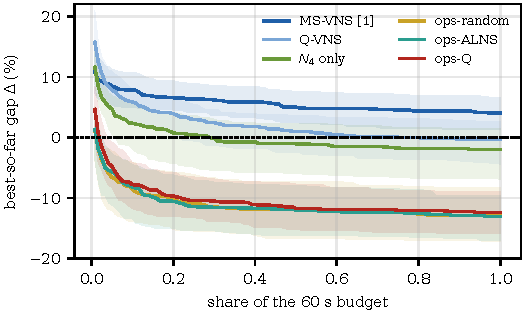
\includegraphics[width=\columnwidth]{figs/fig_results.pdf}
\caption{Best-so-far gap to~\cite{masmoudi2026} over the time budget (median and inter-quartile range of the 150 runs per method).}\label{fig:results}
\end{figure}

\textit{Mechanism.} Fig.~\ref{fig:operators} shows how often each operator pair is chosen and how often it fails. On A0 instances, with small vehicles and tight capacities, greedy insertion leaves a customer without a feasible position in 37--57\% of its moves, against 1--11\% for regret-2 after random, worst or related removal. The agent learns this: its four regret-2 pairs take 71\% of its steps (ALNS: 61\%), which explains its advantage there. On A1/A2 instances, greedy insertion rarely fails (1--2\%), and the only failing operator is route removal (33--40\% infeasible). It is also the only operator that closes a route, and with about six routes a closed route is worth 1000 cost units, more than a 10\% change in distance. Per step, however, route removal looks poor: it improves the current solution in only 60--67\% of its moves, against 93--97\% for the other regret-2 pairs, and fails in a third of them. Since a step earns $+2$ for any improvement and $-1$ for a failure, whatever the size of the gain, the agent learns to avoid route removal (9\% of its steps, against 20\% for ALNS and 25\% for random) and ends with more vehicles. The reward signal rewards \emph{frequent small successes} and does not scale with the size of an improvement. That suits A0, where avoiding wasted moves matters, but it misleads the agent where rare large wins dominate.

\begin{figure*}[t]
\centering
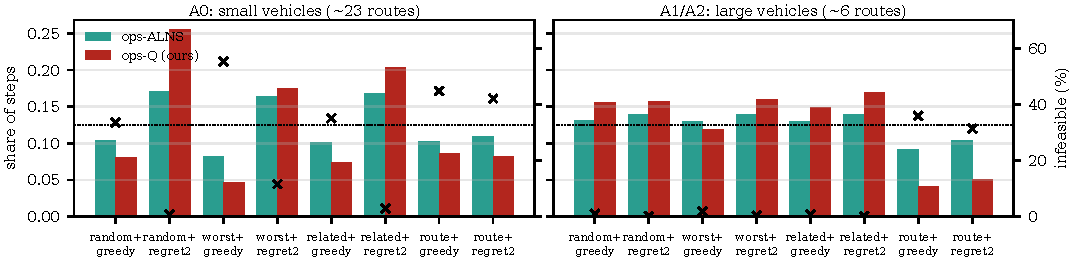
\includegraphics[width=\textwidth]{figs/fig_operators.pdf}
\caption{Share of shaking steps per operator pair for ops-ALNS and ops-Q (bars; the dotted line is the uniform share 1/8) and share of infeasible moves per pair (crosses, right axis), by fleet class.}\label{fig:operators}
\end{figure*}

\subsection{Parameter sensitivity}
Table~\ref{tab:sens} varies one parameter of ops-Q at a time on six instances (one per family, 3 seeds, 60\,s; 144 runs, all feasible). The average gap moves between $-14.6\%$ and $-16.8\%$, a range as wide as the differences between selectors, but only $\alpha=0.05$ differs from the default at the 5\% level (worse, paired Wilcoxon $p=0.012$), and none does after Holm correction over the eight variants. Faster learning helps ($\alpha=0.3$ is best and comes close to ALNS), and slower learning or less exploration ($\alpha=0.05$, $\varepsilon_0=0.1$, $\gamma=0.99$) hurts, which is consistent with the short online horizon. The reward settings confirm the mechanism of Section~V-C. Without the infeasibility penalty, or with a reward for new bests only, route removal on A1/A2 rises from 7.5\% to 19--27\% of the steps, the A1/A2 gap improves from $-19.3\%$ to $-19.8\%$ and $-21.1\%$, and vehicles fall from 7.0 to 6.8 and 6.7, matching the roulette wheel. On A0 the same changes hurt ($-12.7\%$ to $-12.0\%$ and $-10.3\%$). No single per-step reward serves both fleet classes, which is why the trade-off belongs to the reward design rather than to the learning rule.

\begin{table}[t]
\caption{Sensitivity of ops-Q: average gap $\Delta$ (\%) overall and per fleet class, and share of route-removal steps on A1/A2 (6 instances, 3 seeds, 60 s)}\label{tab:sens}
\centering\setlength{\tabcolsep}{4pt}
\begin{tabular}{lrrrr}
\toprule
Setting & $\Delta$ all & $\Delta$ A0 & $\Delta$ A1/A2 & route \% \\
\midrule
Default ($\alpha$=0.1, $\gamma$=0.9, $\varepsilon_0$=0.3) & $-15.99$ & $-12.66$ & $-19.31$ & 7.5 \\
$\alpha=0.05$ & $-14.89$ & $-11.89$ & $-17.89$ & 8.0 \\
$\alpha=0.3$ & $\mathbf{-16.75}$ & $-13.14$ & $-20.35$ & 11.9 \\
$\gamma=0.5$ & $-16.04$ & $\mathbf{-13.18}$ & $-18.91$ & 6.6 \\
$\gamma=0.99$ & $-14.64$ & $-10.25$ & $-19.04$ & 11.0 \\
$\varepsilon_0=0.1$ & $-14.72$ & $-11.93$ & $-17.51$ & 8.8 \\
$\varepsilon_0=0.5$ & $-15.76$ & $-12.57$ & $-18.94$ & 10.1 \\
Reward: new best only & $-15.66$ & $-10.26$ & $\mathbf{-21.06}$ & 27.2 \\
Reward: no penalty & $-15.88$ & $-11.96$ & $-19.79$ & 18.8 \\
\midrule
ops-ALNS (reference) & $-16.97$ & $-12.13$ & $-21.81$ & 19.8 \\
ops-random (reference) & $-16.12$ & $-10.47$ & $-21.77$ & 25.3 \\
\bottomrule
\end{tabular}
\end{table}

\subsection{Discussion: strengths and limitations}
\textit{Operator portfolio.} Its strength is that regret-2 insertion and route removal attack the vehicle term, which dominates~\eqref{eq:obj}; distance also falls by 22\% against MS-VNS, and with it the estimated CO$_2$ emissions (21\% with an illustrative load-dependent model in which a full vehicle emits 30\% more per unit distance than an empty one). Its cost is computational: a destroy-and-repair step is far more expensive than a swap, so only about 136 restarts fit in 60\,s, against 423 for MS-VNS.

\textit{Learned vs.\ adaptive selection.} Q-learning conditions its choice on the search state, needs no hand-set weights, and is the best selector where the main risk is wasting moves (A0). But it is only as good as its reward: a per-step reward that penalizes failure and ignores the size of a gain steers it away from high-risk, high-value operators, and about 2{,}700 online steps per run leave little data to correct this, hence its larger spread. Roulette and uniform choice keep every operator in play and are more robust. The operators matter far more than the mechanism that chooses among them.

\textit{Limitations.} The comparison to~\cite{masmoudi2026} mixes languages and hardware; only the within-study comparisons are on equal terms. The study covers 30 of the 60 instances with 200 customers and one time limit, and the Chen--Shi MCmpt-VRPTW instances used in~\cite{masmoudi2026} are not public, so we could not compare with ALNS on that set.

%=====================================================================
\section{Conclusions}
We reimplemented and validated the MS-VNS of~\cite{masmoudi2026} for multi-compartment routing with reconfigurable vehicles and frigoboxes, and studied learned search control at two levels. At the neighborhood level the decision is nearly trivial: under tight time windows swap and relocate mostly fail, and always applying remove-insert beats both the original score-based policy and Q-learning. Inside remove-insert, a portfolio of four removal and two insertion operators ends 12.5--13.6\% below the published solutions, mainly through about 2.4 fewer vehicles than MS-VNS, and Q-learning selection matches the ALNS roulette wheel and random choice overall. It is best on small-vehicle instances, but its penalty-based reward makes it avoid route removal on large-vehicle instances. Future work includes a reward proportional to the improvement in $f$ (so that closing a route counts as much as it saves), state features that describe the instance (number of routes, capacity tightness), learning across instances rather than online only, and a C++ implementation for a like-for-like comparison with~\cite{masmoudi2026}. Code, notebook and all results: \url{https://github.com/SadiaWaseem/571-Project}.

\section*{Acknowledgment}
Parts of the code and text were drafted with the help of an AI assistant (Claude, Anthropic), as permitted in ISE 571; the authors reviewed all material and are responsible for the content.

\bibliographystyle{IEEEtran}
\bibliography{refs}

\end{document}
